\section{Progettazione Concettuale (Pratica)}
\subsection{Approcci di Progettazione Concettuale}
\begin{itemize}
	\item \textbf{Approccio demand-driven}: Punto focale sono le interviste con il cliente, che devono dare al progettista indicazioni chiare e precise sui fatti, le misure e le gerarchie. Il problema delle sorgenti viene affrontato secondariamente.
	\item \textbf{Approccio supply-driven}: Si può creare lo schema concettuale a partire dalle sole sorgenti. Questo è possibile anche grazie ad un algoritmo che semplifica ed automatizza il tutto. Questo approccio si può utilizzare solo se esiste un DB unico e normalizzato, o comunque se si ha un livello di controllo adeguato sulle sorgenti. Questo sarà anche l'approccio utilizzato per il resto del corso.
\end{itemize}
Le schema del DB riconciliato può assumere tante forme, noi ci concentreremo su schemi E/R e schemi relazionali. Dati questi schemi, la progettazione si articola nei seguenti punti:
\begin{enumerate}
	\item Scelta del fatto;
	\item Per ogni fatto:
	\begin{enumerate}
		\item Costruzione di un \textit{albero degli attributi} $\xleftarrow{}$ questo è il passo automatizzabile;
		\item Editing dell'albero degli attributi $\xleftarrow{}$ parte più soggettiva, ci sono certi gradi di libertà;
		\item Scelta delle dimensioni;
		\item Scelta delle misure;
		\item Creazione dello schema di fatto;
	\end{enumerate}
\end{enumerate}

\subsection{Scelta dei fatti}
I fatti sono concetti di interesse primario per il processo decisionale. Corrispondono ad eventi che accadono in modo \textbf{dinamico}, per esempio VENDITE. Archivi statici o semi statici NON sono buoni candidati (NEGOZIO, REGIONE).

In uno schema E/R, un fatto corrisponde sempre o ad un'entità o ad un'associazione tra più entità. Se lo schema sorgente è relazionale, il fatto corrisponde ad una relazione.

\begin{warn}[Regola euristica per scegliere il fatto:]
	In genere un fatto sta dove ci sono attributi di tipo data, o nelle immediate circostanze.
\end{warn}

Ricordiamo che è sempre possibile reificare un'associazione e farla apparire come un'entità, creando tanto nuove relazioni tante quante erano le entità iniziali. Si creando delle associazioni binarie tra tutte le entità iniziali e quella nuova, con le cardinalità impostate a (1,1) dove mancanti (in uscita dal nuovo fatto) preservando le altre. L'identificatore è composto ed è preso in prestito da tutte le entità iniziali.
\begin{figure}[H]
	\begin{center}
		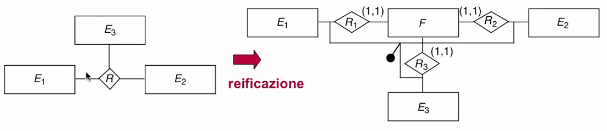
\includegraphics[width=0.6\linewidth]{img/reif.PNG}
		\caption{Reificazione di relazioni in E/R}
	\end{center}
\end{figure}
\noindent A volte esistono più fatti, quando succede in genere si disegnano più schemi di fatto. All'esame in genere la consegna chiederà di sceglierne uno, però scegliendo sempre quello che permette di creare schemi più ampi. Rare volte capita che i fatti da disegnare siano due anche all'esame, ma in questo caso lo schema iniziale è più semplice.

\subsection{Costruzione dell'albero degli attributi}
L'albero degli attributi è un albero in cui:
\begin{itemize}
	\item Ogni vertice (nodo) è un attributo, semplice e composto dello schema sorgente;
	\item La radice è l'identificatore (in caso di ER) o la chiave (in caso di schema logico);
	\item Ogni arco è una dipendenza funzionale.
\end{itemize}

Le dipendenze funzionali sono di due tipi:
\begin{itemize}
	\item Intra-entità: Sono espresse implicitamente, focalizzandosi solo sull'entità. La chiave determina tutti gli altri attributi delle entità. Nella relazione \textit{PRODOTTO(\underline{id}, peso, data, dimensione)}, id determina peso data e dimensione.
	\item Inter-entità: Sono espresse tra più entità, in particolare dove sono presenti cardinalità in uscita che valgono al massimo uno allora esiste una dipendenza funzionale.
\end{itemize}
\begin{info}
	Possiamo vedere l'algoritmo come un gioco in cui una volta scelto il fatto veniamo piazzati all'interno di una stanza che lo rappresenta. Lo scopo è esplorare quante più stanze possibili. Una volta che siamo in una stanza controlliamo ciò che abbiamo intorno (dipendenze intra-entità) e poi ci muoviamo verso un'altra stanza per poi iterare su tutte. Le porte però sono aperte solo se le relazioni in uscita hanno cardinalità (1,1). In risultato non dipende dall'ordine in cui visitiamo le stanze. Alcune passaggi potrebbero essere bloccati, non sempre è possibile obbligatorio visitare tutto lo schema. Potremmo anche entrare più volte nella stessa stanza, ma da punti diversi. In questo caso dovrebbe venirci in mente che potrebbe esserci una gerarchia condivisa o una convergenza.
\end{info}

\subsubsection{Algoritmo pratico}
\begin{enumerate}
	\item Una volta scelto il fatto lo creo e lo chiamo come l'identificatore dell'entità/relazione che lo rappresenta. Questo è il nodo iniziale, ovvero la radice dell'albero.
	\item Poi mi guardo intorno e aggiungo tanti figli, tanti quanti sono gli attributi attraverso cui si creano relazioni intra-entità.
	\item Controllo se ho associazioni in uscita con cardinalità (1,1). Per ciascuno aggiungo un figlio che si chiama come il nome della chiave dell'entità/relazione in cui sono arrivato.
\end{enumerate}

\begin{figure}[H]
	\begin{center}
		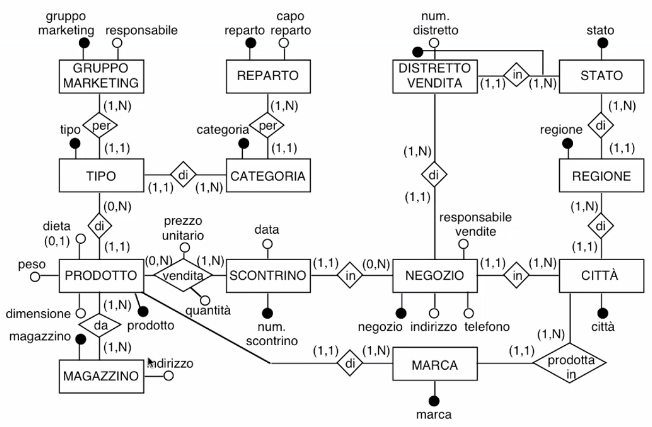
\includegraphics[width=0.8\linewidth]{img/vendite.png}
		\caption{Esempio E/R: Vendite}
	\end{center}
\end{figure}
\noindent Applicando l'algoritmo di arriva ad un risultato simile. In questo caso città è già stato accomunato come concetto utilizzando la gerarchia condivisa. Il ragionamento fatto per capire se si trattasse di gerarchia condivisa oppure convergenza è stato:
\textit{"La città in cui è stato emesso lo scontrino, è anche la stessa in cui viene prodotta la marca dei prodotti acquistati?"}
Essendo la risposta NO non abbiamo vincoli sulle istanze e quindi si tratta di gerarchia condivisa.
\begin{figure}[H]
	\begin{center}
		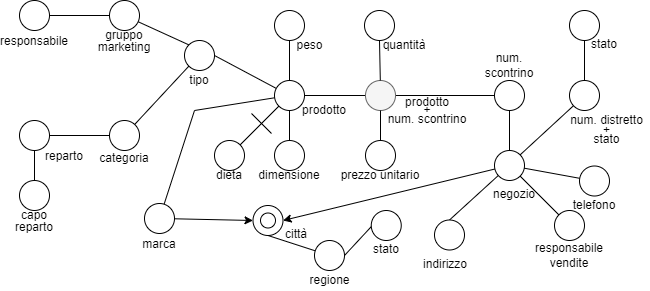
\includegraphics[width=0.8\linewidth]{img/bi-example.drawio.png}
		\caption{DFM: Vendite (dimenticanza convergenza)}
	\end{center}
\end{figure}
\noindent Rimangono alcuni problemi, in questo caso esistono due nodi stato. Possono essere legati? Sì, per esempio anche con una convergenza, se vogliamo porre il vincolo che il negozio deve trovarsi nello stesso stato in cui si trova il distretto di vendita.
\begin{figure}[H]
	\begin{center}
		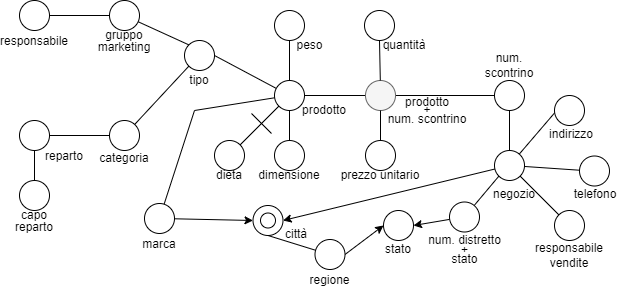
\includegraphics[width=0.8\linewidth]{img/bi-example.drawioconv.png}
		\caption{DFM: Vendite}
	\end{center}
\end{figure}
\begin{warn}
	Da questo algoritmo non traspaiono archi multipli(dovremmo navigare dove ci sono porte chiuse) o attributi cross-dimensionali. L'idea è avere un algoritmo semplice, e aggiungere a posteriori costrutti più complessi solo se i requisiti lo richiedono.
\end{warn}
\subsection{Problemi in progettazione concettuale}
\subsubsection{Attributo su relazione}
Nel caso in cui con l'algoritmo finiamo su una relazione con un attributo come nel caso in immagine, bisogna ragionare a dipendenze funzionali. In questo caso la gravità viene attaccata a Somministrazione, perché è da essa che dipende. Questo avviene perché la relazione è di tipo 1-N quindi abbiamo istanze formate da coppie di Somministrazione e Patologia. Per ognuna ho anche una gravità, quindi ho anche delle triple. Però essendo l'associazione 1-N compare una volta sola la patologia per ogni somministrazione, quindi somministrazione $\xrightarrow{}$ gravità.
\centeredImage{img/attributeonrel.png}{Attributo su relazione}{0.6}
\subsubsection{Cicli}
\begin{figure}[H]
	\begin{center}
		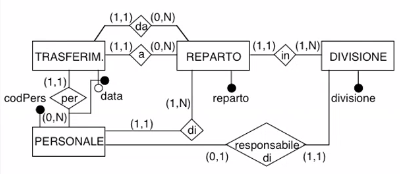
\includegraphics[width=0.5\linewidth]{img/errecur.PNG}
		\caption{Esempio di E/R che creerebbe una ricorsione utilizzando l'algoritmo del DFM}
	\end{center}
\end{figure}
\noindent Ci sono casi in cui può accadere di entrare nella stessa entità o relazione più volte a causa di un ciclo. In questo caso potrebbe venire in mente di utilizzare una gerarchia ricorsiva.
Nel caso in esame, il fatto sono i TRASFERIMENTI. Una possibile soluzione:
\begin{figure}[H]
	\begin{center}
		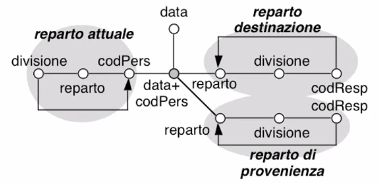
\includegraphics[width=0.5\linewidth]{img/dfmrecurs.PNG}
		\caption{DFM: Soluzione ricorsiva}
	\end{center}
\end{figure}
\noindent Nella pratica la gerarchia ricorsiva è un costrutto piuttosto raro (ha un impatto molto forte nelle fasi successive), quindi se possibile si opta per altre soluzioni...\newline
\begin{figure}[H]
	\begin{center}
		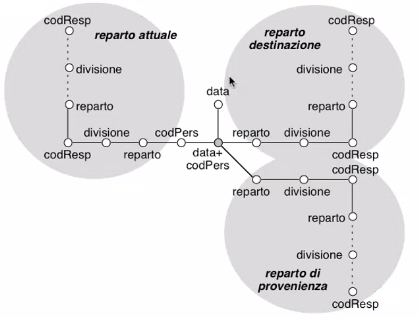
\includegraphics[width=0.5\linewidth]{img/dfmrecsol1.png}
		\caption{DFM: Soluzione del taglio}
	\end{center}
\end{figure}
\noindent La soluzione qui proposta è effettuare qualche giro di ricorsione per poi arrestarsi ad un certo punto (srotolando la gerarchia).
\subsubsection{Gerarchie di specializzazione}
In E/R esistono le gerarchie "is a". Le gerarchie "is a" si possono trasformare in tre modi:
\begin{itemize}
	\item Collasso sulle super-entità;
	\item Collasso sulle sotto-entità;
	\item Sostituire la gerarchia con associazioni binarie.
\end{itemize}
La soluzione che ci interessa è l'ultima perché mantiene al meglio l'informazione. Si creano quindi tante associazioni, con le cardinalità opzionali in uscita dalla super-entità e (1,1) dall'altro lato. L'identificatore della sotto-entità è lo stesso della super-entità.
\begin{figure}[H]
	\begin{center}
		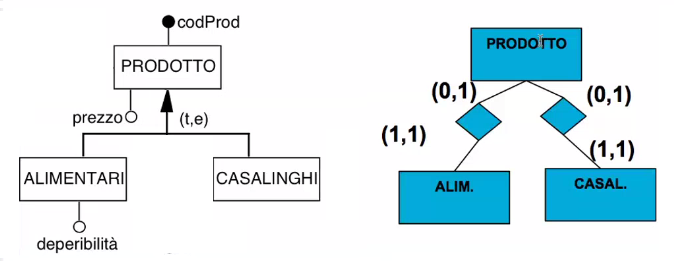
\includegraphics[width=0.8\linewidth]{img/isaconversion.png}
		\caption{Conversione E/R da gerarchia ad associazioni}
	\end{center}
\end{figure}
\begin{warn}
	Navigando verso l'alto non c'è opzionalità, quindi non bisogna, utilizzando l'algoritmo utilizzare il costrutto di arco multiplo. Quello che sicuramente ci sarà sarà una gerarchia condivisa o una convergenza. Gli archi che nel DFM però sono archi 1-1 e quindi andranno gestiti in qualche modo.
\end{warn}
\subsubsection{Associazioni n-arie}
Anche se le associazioni n-arie sono per noi porte chiuse esistono i casi delle false n-arie. In questo caso lo schema è rappresentato in modo sbagliato, perché quell'associazione si può rappresentare come due relazioni.
\begin{figure}[H]
	\begin{center}
		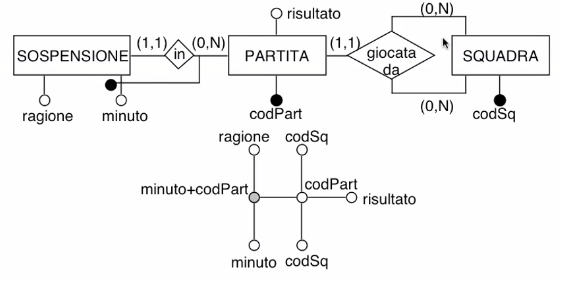
\includegraphics[width=0.8\linewidth]{img/falsetern.PNG}
		\caption{Conversione E/R da falsa ternaria}
	\end{center}
\end{figure}

\subsubsection{Attributi composti}
Gli attributi composti vengono trattati come entità e quindi vanno rappresentato sia il nodo dell'attributo composto che tutti i suoi componenti come figli. Anche in caso di identificatori composti essi vanno sempre tutti rappresentati come nel secondo esempio in immagine.
\begin{figure}[H]
	\begin{center}
		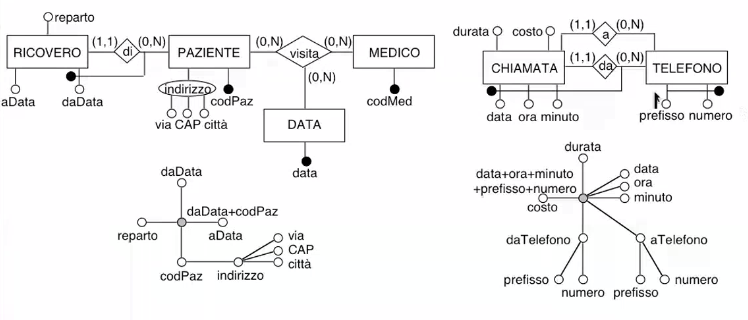
\includegraphics[width=0.9\linewidth]{img/composti.PNG}		\caption{DFM con attributi composti}
	\end{center}
\end{figure}

\subsection{Editing dell'albero}
Non tutti gli attributi sono d'interesse per il Data Mart. Alcuni nodi potrebbero non servire e quindi possono essere eliminati. Esistono due modi per eliminarli:
\begin{itemize}
	\item \textbf{Potatura}: Si eliminano un nodo e tutti i suoi figli.
	\item \textbf{Innesto}: C'è un nodo che ha un livello di granularità non interessante ma che ha figli con un livello di granularità interessante. In questo caso desideriamo mantenere i figli.
\end{itemize}

\begin{figure}[H]
	\begin{center}
		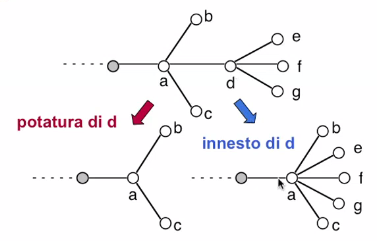
\includegraphics[width=0.4\linewidth]{img/potinnest.PNG}		\caption{Editing dell'albero: Potatura ed Innesto}
	\end{center}
\end{figure}
\noindent Le dipendenze funzionali dirette dell'albero di partenza sono:
\newline
a $\xrightarrow{}$ b, a $\xrightarrow{}$ c, a $\xrightarrow{}$ d, d $\xrightarrow{}$ e, d $\xrightarrow{}$ f, d $\xrightarrow{}$ g\newline
Ma ce ne sono anche di transitive:\newline
a $\xrightarrow{}$ e, a $\xrightarrow{}$ f, a $\xrightarrow{}$ g.\newline
Come possiamo notare, le dipendenze funzionali sono tutte preservate in entrambi i casi, al massimo vengono completamente rimosse.\newline
Se si elimina un nodo opzionale l'opzionalità è ereditata da tutti i figli.\newline
Eliminare un figlio diretto della radice implica aggregare, e quindi avere un livello più grossolano di granularità del fatto. In questo caso si aggiunge sempre una misura al fatto, che indica il conteggio.\newline
Altre manipolazioni sono lo spostamento di un arco intero come nel seguente caso:
\centeredImage{img/spostamento archi.PNG}{Editing dell'albero: Spostamento archi}{0.6}
\noindent Le dipendenze funzionali del DFM a sinistra sono:\newline
a $\xrightarrow{}$ b, b $\xrightarrow{}$ c, a $\xrightarrow{}$ c\newline
Nello schema di destra invece:
a $\xrightarrow{}$ b, a $\xrightarrow{}$ c\newline
Passare da una gerarchia profonda ad una gerarchia larga significa rimuovere dipendenze funzionali. Viceversa passare da una gerarchia larga ad una gerarchia profonda significa aggiungere dipendenze funzionali.
\begin{warn}[Per esame:]
	Nei compiti a volte si dice di normalizzare lo schema sorgente se non lo è. Un approccio potrebbe essere farlo all'inizio, ma è un metodo lento e error-prone. Molto più pratico è svolgere normalmente l'esercizio ed applicare/rimuovere le dipendenze funzionali attraverso il metodo appena illustrato.
\end{warn}
A volte possono essere presenti associazioni uno a uno (si tratta di un caso particolare di una molti a molti). Esempio di una relazione:\newline
R(\underline{kr}, a)\newline
S(\underline{kr}: R, b)\newline
\centeredImage{img/arcounoauno.PNG}{Associazione uno ad uno}{0.25}
\noindent In fase di costruzione dell'albero ci segnamo quindi le associazioni uno ad uno perché poi dovremo rimuoverle in qualche modo. Questi tipi di archi nel DFM devono sparire. Ci sono tre modi per liberarsene:
\begin{itemize}
	\item Tramutandoli in attributi descrittivi. In questo caso tutti i figli vanno persi.
	\item Facendo un innesto, ovvero rimuovendo l'associazione uno ad uno. In questo caso i figli si attaccano al livello in cui era l'attributo eliminato.
	\item Effettuare uno swap. Esistono alcuni casi in cui la chiave utilizzato è un surrogato. Se esiste un attributo che può prendere le veci della chiave allora i due attributi dipendono l'uno dall'altro e quindi si possono scambiare. Questo rende anche possibile eliminare il surrogato.
\end{itemize}
\begin{warn}[]
	In uno schema relazionale anche se la strada sembra chiusa in un verso in una relazione uno a uno in realtà non lo è, solo che entrando da un verso l'arco è normale, entrando dal verso opposto l'arco è opzionale. Vedi esempio dei voli.
\end{warn}
\subsection{Scelta delle dimensioni}
Le dimensioni vengono scelte nell'albero degli attributi tra i vertici figli della radice. La scelta è cruciale perché definisce la granularità degli eventi primari. Gli attributi possono corrispondere ad attributi discreti o ad intervalli. La scelta delle dimensioni però è stata univocamente determinata dalla maniera in cui è stato fatto l'editing.
\subsection{Creazione dello schema di fatto}
La creazione dello schema di fatto è ora molto semplice, perché a partire dall'albero degli attributi si ottiene lo schema con pochissimi passaggi.
\begin{itemize}
	\item Si rimuove la radice dell'albero e si inserisce il rettangolo col nome del fatto;
	\item Le misure finiscono nel secondo scompartimento del fatto. Se non ce ne sono si specifica (COUNT), sta ad indicare che per fare aggregazione faremo dei conteggi;
	\item I nodi che non sono stati scelti né come misure né come dimensioni tendenzialmente spariscono
	\item In questo momento ci poniamo anche il problema degli attributi cross-dimensionali e degli archi multipli. Se l'utente finale desidera effettuare analisi aggiuntive su qualcosa che non è sull'albero degli attributi questo è il momento di aggiungere questi costrutti.
	\item Per ogni coppia misura-dimensione si specifica se la misura è additiva oppure no.
\end{itemize}
\subsection{Carico di lavoro}
Sul DFM é possibile annotare le query, per esempio, la seguente immagine rappresenta il \textit{"Totale della quantità venduta per i diversi tipi di prodotto, in ogni settimana e città ma solo per i prodotti alimentari"}.
\centeredImage{img/querydfm.png}{Esempio di Query raffigurabile su DFM}{0.5}
\noindent Quando il carico di lavoro aumenta troppo o l'interesse dell'utente cambia si effettua un'operazione di tuning per risolvere. Nella realtà non si tocca niente finché tutto funziona, solo una volta che gli utenti cominciano a lamentarsi della prestazione si agisce.\newline
Non tutti gli utenti sono uguali, alcuni hanno esigenze di accesso ed utilizzo di dati specifici e non devono interagire con altri. Per rappresentare i ruoli e classificarli in gruppi (profilazione) si può utilizzare UML, nello specifichi il diagramma dei casi d'uso.\newline
Uno degli scopi può essere per esempio impedire a determinate classi di utenti di poter visualizzare dati sensibili, o vietare loro di poter effettuare determinate operazioni.

\newpage
